\documentclass[letterpaper,10pt]{article}

%\setlength{\parindent}{0in}
%\usepackage{fullpage} 
\usepackage{amsmath}
\usepackage{amssymb}
\usepackage{enumerate}
\usepackage{graphicx}
\usepackage[table]{xcolor}
\usepackage{dcolumn}
\oddsidemargin 0.0in
\textwidth 6.5in
\newcolumntype{.}{D{.}{.}{-1}}
\newcommand*{\myalign}[2]{\multicolumn{1}{#1}{#2}}

%opening
\title{Homework}
\author{Steve Mazza}
\date{July 22, 2013}

\begin{document}
\maketitle

\section*{Homework 2}
\subsection*{Problem 1}
\begin{align*}
	\dfrac{s\omega(s)}{0.25} &= \dfrac{2.5(s+2)}{(s+5)(s+1)^2} \\
	\omega(s) &= \frac{5}{8}\left(\dfrac{s+2}{s(s+5)(s+1)^2}\right) \\
	\omega(s) &= \frac{5}{8}\left(-\dfrac{7}{16(s+1)} + \dfrac{3}{80(s+5)} - \dfrac{1}{4(s+1)^2}+ \dfrac{2}{5s}\right) \\
	\omega(t) &= \frac{5}{8}\left(-\frac{1}{4}te^{-t} + \dfrac{3e^{-5t}}{80} - \dfrac{7e^{-t}}{16} + \frac{2}{5}\right)
\end{align*}

\subsection*{Problem 6}
\begin{center}
	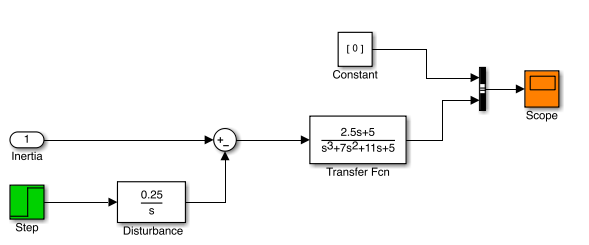
\includegraphics[scale=0.75]{simulink-h2.png}
\end{center}
See the attached file, \texttt{homework2.slx}.

\section*{Homework 3}
\subsection*{Problem 2}
\begin{align*}
	\dfrac{C(s)}{R(s)} &= \dfrac{1}{Ts+1} \\
	C(s) &= \frac{1}{s}\left(\dfrac{1}{Ts+1}\right) \\
	C(s) &= \frac{1}{s} - \dfrac{T}{Ts+1} \\
	C(s) &= \frac{1}{s} - \dfrac{1}{s+(1/T)} \\
	c(t) &= 1 - e^{-1/T} \\
	0.98 &= 1 - e^{-1/T} \\
	0.02 &= e^{-1/T} \\
	ln(0.02) &= -\frac{1}{T} \\
	T &= -\dfrac{1}{ln(0.02)} \\
	T &\approx 0.2556 \mbox{\ minutes} \\
	&\approx 15.3373 \mbox{\ seconds}
\end{align*}

\subsection*{Problem 3}
Based on the information supplied, we determine that $J = 1$ and $B = 14$.
Next we use the equation $\dfrac{K}{J} = \omega_{n}^{2}$ to determine that $K=\omega_{n}^{2}$.  Finally we use the equation $\dfrac{B}{J}=2\zeta\omega_{n}$ as follows:
\begin{align*}
	B &= 2\zeta\omega_{n} \\
	7 &= \zeta\omega_{n} \\
	7 &= 0.7\omega_{n} \\
	10 &= \omega_{n} \\
	10^2 &= K \\
	100 &= K
\end{align*}

\subsection*{Problem 4}
We use the information given to determine the following three sets of inequalities in terms of $\omega_{d}$ and $\sigma$.

Given what we know about \emph{percent overshoot}:
\begin{align*}
	M_{p} &\leq e^{-(\sigma/\omega_{d})\pi} \\
	ln(0.05) &\leq -\left(\dfrac{\sigma}{\omega_{d}}\right)\pi \\
	\dfrac{ln(0.05)}{\pi} &\leq -\dfrac{\sigma}{\omega_{d}}
\end{align*}

Given what we know about \emph{settling time}:
\begin{align*}
	t_{s} &< \dfrac{4}{\sigma} \\
	4 &> \dfrac{4}{\sigma} \\
	\sigma &> 1
\end{align*}

Given what we know about \emph{peak time}:
\begin{align*}
	1 &> \dfrac{\pi}{\omega_{d}} \\
	\omega_{d} &> \pi
\end{align*}

Optionally, we locate the poles with the equation $ s_{1, 2} = -\sigma \pm j\omega_{d}$.  Then we plot these inequalities to determine the permissible area for poles of $T(s)$.

\begin{center}
	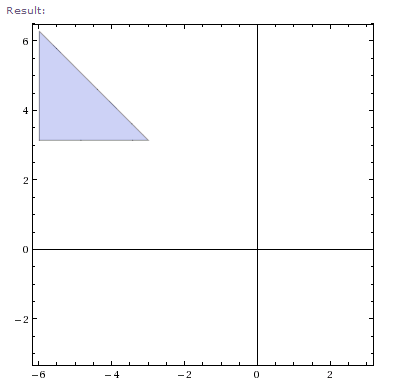
\includegraphics[scale=0.5]{plot-h02-02}
	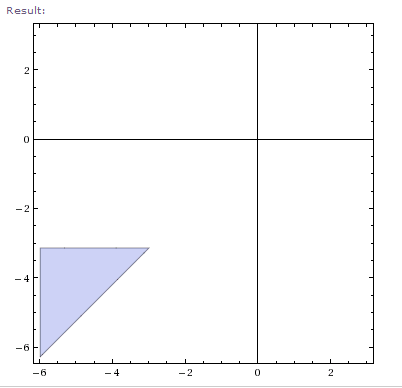
\includegraphics[scale=0.5]{plot-h02-01}
\end{center}

\end{document}